\documentclass[twoside,a4paper]{refart}
\usepackage{makeidx}
\usepackage{ifthen}
\usepackage{graphicx}
\usepackage[colorlinks=false,allbordercolors={1 1 1}]{hyperref}
\usepackage{minted}

\def\bs{\char'134 } % backslash in \tt font.
\newcommand{\ie}{i.\,e.,}
\newcommand{\ra}{$\rightarrow$}
\DeclareRobustCommand\cs[1]{\texttt{\char`\\#1}}

\renewcommand{\abstractname}{Introduction}

\title{\mdseries \textbf{ItATMIS} \\ \textbf{It}erative \textbf{A}nnotation and \textbf{T}raining for \textbf{M}edical \textbf{I}mage \textbf{S}egmentation}
\author{Jacob Johnson, MS}

\date{}
\emergencystretch1em  %

\pagestyle{myfootings}
\markboth{ItATMIS User Guide}%
         {ItATMIS User Guide}

\makeindex 

\setcounter{tocdepth}{2}

\begin{document}
\maketitle

\begin{abstract}
        This document is used as a helpful guide for using the medical image segmenation application. Any issues not covered here should be directed to \href{mailto:jmjohnson33@wisc.edu}{Jacob Johnson}.
\end{abstract}

\tableofcontents

\newpage

\index{Getting started}\section{Getting started}
%%
\index{Requirements}\subsection{Requirements}
Currently, ItATMIS is only supported on Linux. It was developed in a Python 3.5 Anaconda environment. Using the application in other settings is not supported and can have variable success.

ItATMIS is meant to be used with an installed Nvidia GPU. Depending on the size of your images, the GPU must have on the order of 8 GB of memory. ItATMIS will be most effective if a high end GPU is used, such as GTX 1080 Ti or Titan Xp. A compatible version of CUDA and CuDNN must already be installed. 
%%
\index{Installation}\subsection{Installation}
Install the Python package requirements listed in \mintinline{bash}{itatmis_requirements.txt}, either manually or using PyPi, as in:
\begin{minted}{bash}
	pip install itatmis_requirements.txt
\end{minted}
inside your conda environment.

\index{ItATMIS interface}\subsection{ItATMIS Interface}

The initial ItATMIS interface is shown below. It consists of
\begin{itemize}
	\item A central area containing 3 display panels which will contain the axial, coronal, and sagittal views of images once loaded
	\item A slice selection slider on the left side of the interface
	\item A toolbar across the top of the interface, which includes buttons for saving/loading an ItATMIS project and tools for interacting with the segmentation
	\item A panel in the upper right of the interface allows more interaction with the segmentation process.
	\item A set of panels on the lower right side. These contain buttons for selecting data for segmentation, starting the training, and for evaluating the deep learning model on the current subject. Two text displays contain a list of the files that are included in the project and any messages from the program. 
\end{itemize}

\hspace{1cm}
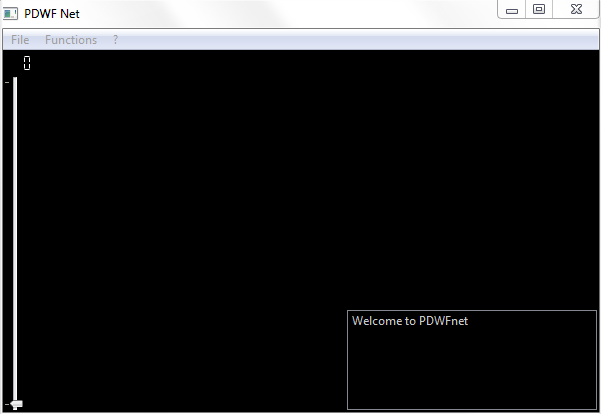
\includegraphics[width=.8\textwidth]{InitialInterface.png}

\index{Quick Start}\subsection{Quick Start}

An example procedure for starting a new ItATMIS project is:

\begin{enumerate}
	\item Start ItATMIS
	\item Click `Select Data...' to open the data selection interface
	\item Click `Select NifTI Files...'
	\item Navigate to the directory containing your NifTI files that need to be segmented
	\item Select the first file of the sequence and click 'Open'
	\item Set the number of classes using the arrow buttons, if you are segmenting more than 1 class
	\item Click `Set Selected Images'
	\item The first subject in the list will automatically be loaded and displayed
	\item Manually segment the images as desired. Left click is add to segmentation and right click is erase. Change classes (if more than 1) 			using the selector on the upper left side of the interface
	\item Scroll through the image stack using the slider on the left until all images are segmented
	\item Click `Train' to begin training the deep learning model
	\item The training will begin in the background. Double click another subject from the list on the right side to load it.
	\item While the training is running, begin manually segmenting the new subject. Once the training is complete, the model will 					automatically evaluate any slices you have not annotated yet.
	\item If the segmentation is not satisfactory, it can be cleared slice by slice or the entire 3D mask using the Clear button on the toolbar
	\item Once the second subject is completely segmented, click `Train' again to train the deep learning model with the new data included
	\item Repeat the process until the deep learning model provides satisfactory results
	\item At any time after the initial training, click `Evaluate Current Subject' to get the results of the deep learning model on the subject 			currently loaded. The model will only evaluate slices that do not have any annotations already.

\end{enumerate}

%%%%%%%%%%%%%%%%%%%%%%%%%%%%%%%%%%%%%%%%%%%%%%%%%%%%%%%%%%%%%%%%%%%%
\newpage
\section{Images}

\index{Image Handling}\subsection{Image Handling}


ItATMIS is currently designed to accept 3D images in the form of a single NifTI file for each subject. There are many conversion tools available, e.g. \textbf{dcm2nii} for Matlab, that can process DICOM images and return them in the desired form.

4D NifTIs are not currently supported. If you wish to use 4D images, split them into individual 3D NifTI files.

The NifTI files are to be stored in a single directory, which will act as the working directory for the ItATMIS project. Preferably, only the NifTI files of interest and nothing else will be stored in this directory so as not to interfere with ItATMIS file reading and saving.

Once the ItATMIS project is complete, the masks will be stored in a sub-directory of the image directory, also in NifTI format.


\index{Importing Images}\subsection{Importing Images}

Once your images are ready for import, run ItATMIS and click `Select Data...'. The following importing interface will appear.

\hspace{2cm}
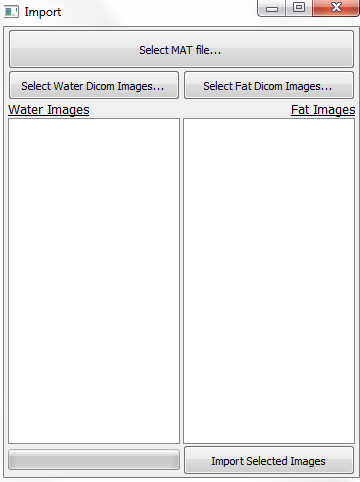
\includegraphics[width=.6\textwidth]{ImportGUI.PNG}

Click `Select NifTI Files...' and nagivate to the directory of the images you wish to import. Select any image in the directory and click `Open'; the list of NifTI images in that directory will be displayed.

You can remove files from this list by right clicking and selecting `Remove from Import'. Once the images are selected, the file list cannot be changed without starting a new project.

If you wish to segment more than 1 class (i.e. 1 class for lungs, 1 class for heart, etc.) then increase the number of classes using the arrows. Currently, a maximum of 6 classes is supported. Using fewer classes will give better deep learning results.

Once you are ready, click `Set Selected Images'. The first subject will be loaded into the display and will be ready for segmentation. The list of files will be displayed on the right side of the interface. The current subject will be highlighted. At any time, double-clicking one of the files will save the current subject and load the selected one.

Selected data in this way begins an ItATMIS project. The project can now be saved using the save button on the toolbar.


\index{Save and Load Project Data}\subsection{Save and Load Project Data}

At any point after images are selected, you can generate a ItATMIS project file by selecting the Save button in the upper left of the interface. You will be prompted to choose a location and filename for the data file. All pertinent aspects of the segmentation will be saved in a specifically formatted .HDF5 file, allowing you to pick up where you left off. You can reload the project using the adjacent Load button.



%%%%%%%%%%%%%%%%%%%%%%%%%%%%%%%%%%%%%%%%%%%%%%%%%%%%%%%%%%%%%%%%%%%%

\section{Segmentation}

%%%%%%%%%%%%%%%%%%%%%

\index{Interface Basics}\subsection{Interface basics}

\marginlabel{Drawing}
Click and drag the cursor over the main view plane to make an annotation. Click and drag with the right mouse button to erase.

\marginlabel{Zooming}
Hold Ctrl while scrolling the mouse wheel to zoom in or out.

\marginlabel{Window/Level}
Adjust the window and level by clicking and dragging with the middle mouse button (scroll wheel button).

\marginlabel{3-plane scrolling}
The main, axial viewing window is the only window for editing annotations. However, the coronal and sagittal view windows can be used to pinpoint a certain location by clicking or dragging the crosshairs.


\index{User Interface}\subsection{User Interface}

\hspace{-1.6in}
\begin{minipage}{1.35\textwidth}

\includegraphics[width=.3\textwidth]{CorrectionsToolbar.PNG}

\normalsize{Each of these tools are described below}
\end{minipage}\\[1em]

\normalsize

\index{Reset View}\marginlabel{Reset View}
This button will reset the viewing modules to their default settings, including window/leveling, panning, and zooming.

\index{Clear Mask}\marginlabel{Clear Mask}
This button will clear the current mask. You will be given of clearing the current slice or the entire 3D mask. This is helpful if the deep learning model is not yet providing helpful annotations and you need to clear them out.

\index{Undo}\marginlabel{Undo (Ctrl + Z)}
This button undos the last brush stroke. Up to 10 of the last annotations are stored.

\index{Quick Select Mode}\marginlabel{Quick Select Mode (P)}
Click this button to enable quick select mode, an enhanced drawing interface that allows you to quickly annotate well-defined regions in images. The method relies on superpixel segmentation using the watershed approach. It will be most effective when the region you are annotating has highly contrasting edges with its surroundings, e.g. the lungs. It may be less effective in regions with lower constrast.

Quick select mode works for both drawing and erasing.

\large{Other tools and settings}

\normalsize

\marginlabel{Slice Slider}
Slices can be scrolled through using the slider on the left, by moving the scroll wheel on your mouse, or by pressing the +/- keys on your keyboard. The current slice number is indicated at the top of the slider.

\marginlabel{Brush Size}
The current brush radius (in pixels) is shown in the panel on the upper right of the interface. You can change the brush radius using the slider. Brush size can also be increased by pressing the `[' key and decreased by pressing the `]' key.

\textbf{Note:} The circular brushes drawn on the screen will line up with the selection being made. The cursors will change size when zooming is performed, but there can be inconsistencies with certain zoom settings and pixel resolutions between the actual footprint of the brush and the size of the cursor. 


%%%

\index{Using ItATMIS}\subsection{Tips for using ItATMIS}
Here are some tips to on how to properly use this application.

\index{Holes}\marginlabel{Holes}
The application does not allow holes in the mask. Any hole that would be made by either an addition or erasure from the mask will automatically be filled in.

\index{Quick Select Strategy}\marginlabel{Quick Select Strategy}
Using quick select mode is not effective for all regions or images being annotated. However, if it suits your task, the following strategy is recommended.

First, highlight the desired region with quick select mode on. Make sure the entire region is highlighted, even if it means extraneous regions are highlighted as well.

Next, turn off quick select mode. Erase the extraneous regions using regular brush strokes, until the annotation is as desired.

This strategy has been found to be efficient and effective at getting a high quality segmentation.



%%%%%%%%%%%%%%%%%%%%%%%%%%%%%%%%%%%%%%%%%%%%%%%%%%%%%%%%%%%%%%%%%%%%%%

\printindex

\end{document}
